\section{Endpoint probes with a persistent vertex cache}
\label{app:endpoint}
The finite-termination result of Corollary~\ref{face:endpoint} does not
imply a practical advantage outside its full-solution-face assumptions.
We evaluated 108 matched dataset/radius/start configurations from the
Seoul and Metro count-data tasks with three methods: ordinary
backtracking, endpoint tests at every update, and tests at indices
$k+1=2^j$, $j=0,1,\ldots$. These are configurations from two datasets,
not independent statistical samples. All methods start from the same
source and use $M=U_0/D^2$; the endpoint Armijo coefficient is
$\sigma=1/2$.

\paragraph{Persistent cache and paid-budget protocol.}
Each method, including its ordinary baseline, has its own persistent
cache. Only values at exactly represented signed-coordinate vertices
are shared between queries: the cache key records dimension, coordinate
and sign, and membership requires exact coordinate equality to the
radius and exact zeros elsewhere. Nearby points do not share a key.
The deterministic Float64 objective and operation order are fixed;
cache hits reuse that value without another paid function call.
Nonvertex values, gradients and full LMOs remain separately charged.
A failed endpoint test uses the unchanged quadratic-backtracking
fallback and tie rule. At the budget of 1000 paid objective calls, the
reported source prefix is the last source whose cumulative paid
function count is at most 1000; a trial that crosses the budget does
not make the subsequent source affordable. Other oracle types are
unrestricted in this single-oracle comparison.

\begin{table}[htbp]
\centering
\small
\caption{Persistent-cache endpoint probes: certificate ratio $U_{\rm probe}/U_{\rm ordinary}$ at 1000 paid objective evaluations, over 108 paired configurations.}
\label{endpoint:table}
\begin{tabular}{lrrrr}
\toprule
Probe schedule & Median ratio & Better $>1\%$ & Worse $>1\%$ & Within $1\%$ \\
\midrule
Dense & 1.004798 & 0 & 35 & 73 \\
Dyadic & 1.000727 & 0 & 12 & 96 \\
\bottomrule
\end{tabular}
\end{table}


No endpoint test was accepted in any of the 324 runs. At the common
1000-call source prefix, the dense persistent-cache median certificate
ratio was $1.00479805149$; 0, 35 and 73 configurations were respectively
better by more than 1\%, worse by more than 1\%, and within 1\% of the
ordinary baseline. The corresponding dyadic median was $1.00072704517$,
with counts 0, 12 and 96. A paired audit of the 216 dense/dyadic versus
ordinary paths found 106623 matching sources and 106407 matching
transitions, including objective, gap, certificate, accepted curvature
and step. At equal update counts, every paid-function difference was
between zero and the number of vertices; the maximum observed extra
cost was 17 calls.

Ridge regularization makes the Poisson objective strictly convex.
In every task, numerical comparison placed each vertex above a better
feasible reference point, locating the unique optimum away from the
vertices. These tasks
therefore do not satisfy~\eqref{face:exposed}; in particular, their
minimizers do not form the full exposed solution face assumed by the
termination theorem. The results measure the cost of unsuccessful
probes outside that regime. They establish neither a wall-clock speedup
nor better progress per mathematical update.

\paragraph{A cache bound at equal update counts.}
If all added probes are rejected, the initial state and fallback rule
coincide, and both methods permanently cache exact vertex values, then
for every fixed number $K$ of updates,
\[
 0\le N_f^{\rm probe}(K)-N_f^{\rm ordinary}(K)\le |V|.
\]
Indeed, all fallback iterates and nonvertex queries coincide. Each
vertex is paid for at most once, and the difference counts vertices
queried only by the probing method. This statement concerns equal
update counts; Table~\ref{endpoint:table} instead fixes a paid-function
budget.

\subsection{An exact check within the exposed-face assumptions}
\paragraph{An exposed-face mechanism check.}
To complement the out-of-regime count-data controls, we independently
implemented the exact example of Section~5.1 using rational arithmetic.
The study contains 54 exact runs: six ordinary baseline runs and 48
endpoint-probe runs. The six starts use
$t_0\in\{1,1/2,1/4\}$ and $z_0\in\{-1/3,1/3\}$. The probe runs
vary over $\sigma\in\{1/2,9/10,99/100,1-2^{-20}\}$ and dense or
dyadic schedules. Ordinary FW remains nonterminal at the
64-update audit cap; the manuscript's analytic recurrence describes
its infinite continuation. All 48 probing runs attain $U=0$ exactly,
within at most 16 updates. The 222 sources preceding an accepted
endpoint match their ordinary counterparts exactly in iterate,
objective, gap and scalar certificate. A persistent cache pays for at
most two distinct endpoint values in these runs. These are variations
of one analytic example, not independent datasets or evidence of a
general practical advantage. Source, full traces and a SHA-256 manifest
are supplied in the companion archive.

\begin{figure}[htbp]
\centering
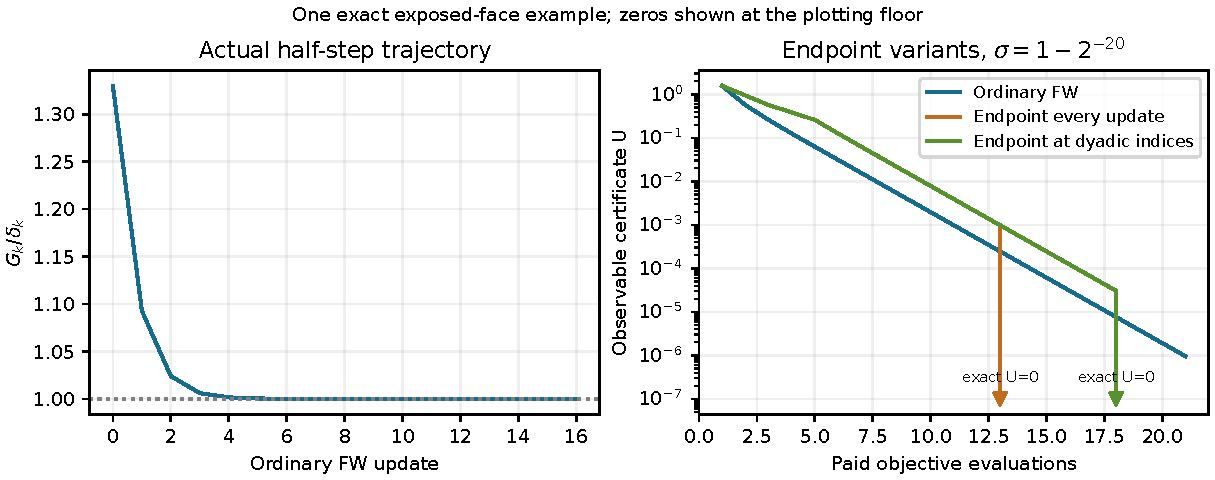
\includegraphics[width=\textwidth]{figures/exposed_face_mechanism.pdf}
\caption{Exact exposed-face study with 54 runs: six ordinary baselines
and 48 dense or dyadic endpoint-probe runs. Left: the half-step
trajectory has $G_k/\delta_k\to1$. Right: dense and dyadic endpoint
tests reach exact $U=0$; zeros are marked at a display floor of
$10^{-7}$. The ordinary run remains nonterminal. The horizontal axis
counts paid objective evaluations; this illustration does not give a
general practical ranking. Source, traces and SHA-256 manifest are
available in the companion archive.}
\label{fig:face-mechanism}
\end{figure}
